% CARE-LG paper -- IEEE conference template, 6 pages + references.  main_final.tex (final paper).
% Numbers: results/tables (NHANES 1999-2023 from the full rerun, results/run_full_nhanes; other datasets unchanged from report_v3),
% see results/FULL_RERUN_CHANGES.md. Source tables are named in % comments. Red \todo{} = author decision or check needed.
% The earlier eICU/CARE-N v2 draft is kept unchanged in archive/experiments_caren/paper/.
\documentclass[conference]{IEEEtran}
\IEEEoverridecommandlockouts
\usepackage{cite}
\usepackage{amsmath,amssymb,amsfonts,amsthm}
\usepackage{graphicx}
\usepackage{booktabs}
\usepackage{multirow}
\usepackage{xcolor}
\usepackage{url}
\usepackage[hidelinks]{hyperref}

\newcommand{\todo}[1]{\textcolor{red}{[TODO: #1]}}
\newcommand{\method}{CARE-LG}
\newtheorem{proposition}{Proposition}

\begin{document}

% TODO: working title; final title to be decided.
\title{\method: Tiered, Ontology-Grounded Actionable Recourse for Cardiovascular Risk with Certified Real-Patient Paths and Certified Infeasibility}

\author{
\IEEEauthorblockN{Roozi \todo{full name}, Amaljith S J, Haridev N, Ananthu P S}
\IEEEauthorblockA{Department of Computer Science and Engineering\\
TKM College of Engineering, Kollam, Kerala, India\\
\todo{emails}}
\and
\IEEEauthorblockN{Reshma Sheik}
\IEEEauthorblockA{Department of Computer Science and Engineering\\
TKM College of Engineering, Kollam, Kerala, India\\
\todo{email}}
}

\maketitle

\begin{abstract}
Counterfactual recourse methods either search over real patients, which gives plausible but often unavailable recourse, or generate synthetic points, which are almost always available but often clinically inadmissible. We present \method{}, which gives every high-risk patient one of three outcomes: (1) a \emph{certified} path to a real lower-risk patient, checked on recorded values and by an answer-set-programming certificate; (2) an ontology-guided synthetic counterfactual, used only when (1) is provably impossible; or (3) a certified statement that no real-patient recourse exists, with the closest miss. Patient-specific guideline targets and contraindications are inherited down the ICD-10-CM hierarchy, and recommendations escalate from lifestyle to one drug to combination therapy while skipping drugs the patient already takes. On 32,786 adults pooled from eleven NHANES cycles (1999--2023; 15,002 high-risk test patients over 5 seeds), 96.4\% of high-risk patients receive admissible recourse, 63.1\% through a certified real patient, with zero real-value violations on 9,471 certified paths and zero contraindicated recommendations. The best of six baselines reaches 66.4\%; FACE, Growing Spheres, DiCE and C-CHVAE reach validity mostly by changing immutable attributes or age. Removing ontology inheritance lets contraindicated drugs through, removing escalation halves guideline-consistent ordering, and real-patient targets stay valid under model retraining far more often than synthetic ones (84.9\% vs.\ 63.5\%). An audit shows that infeasibility is not evenly shared: tier~1 reaches 89.5\% of high-risk women but 48.2\% of men, and tier-3 cases occur only in men.
\end{abstract}

\begin{IEEEkeywords}
explainable AI, algorithmic recourse, counterfactual explanations, neurosymbolic AI, answer set programming, clinical ontology, cardiovascular risk, NHANES
\end{IEEEkeywords}

% =====================================================================
\section{Introduction}
% =====================================================================
Ten-year cardiovascular risk estimates such as the Pooled Cohort Equations (PCE)~\cite{goff2014pce} drive prevention decisions, and machine-learned risk models increasingly sit beside them. A risk score says who is at risk; clinicians also need to know what would lower it, in terms consistent with guidelines~\cite{tonekaboni2019clinicians}. Counterfactual explanations~\cite{wachter2018counterfactual} and algorithmic recourse~\cite{ustun2019actionable,karimi2022survey} answer this question by proposing a change to the patient's features after which the model predicts lower risk.

Existing generators fall into two families with opposite failures. \emph{Real-data} methods such as FACE~\cite{poyiadzi2020face} return recorded individuals, which are plausible, but the nearest low-risk person usually differs from the patient in sex, is younger, or has worse values elsewhere. \emph{Synthetic} methods such as DiCE~\cite{mothilal2020dice}, Growing Spheres~\cite{laugel2018growing}, C-CHVAE~\cite{pawelczyk2020cchvae} and Wachter-style optimisation~\cite{wachter2018counterfactual} almost always find a point, but without clinical rules the point may change immutable attributes, reverse time, or ask for implausible values. Neither family says what to do when no admissible recourse exists, although recourse verification~\cite{kothari2024reach} shows that such patients are common and that hiding them is itself a harm. Finally, clinical knowledge rarely enters these methods: nothing stops a non-selective beta-blocker being recommended to a patient with asthma.

\method{} combines both families with symbolic clinical knowledge and makes failure explicit. Our contributions are:
\begin{enumerate}
  \item \textbf{Tiered recourse with certificates.} A certified path to a real patient (tier~1); an ontology-guided synthetic counterfactual only when tier~1 is provably infeasible (tier~2); otherwise a certified statement of infeasibility with its closest miss (tier~3). Under source-relative admissibility, every tier-1 failure is an exhaustive certificate over all training patients.
  \item \textbf{Ontology-compiled rules with inheritance.} ICD-10-CM concepts derived from survey and prescription data activate patient-specific targets (e.g.\ blood pressure below 130/80 with diabetes or CKD) and contraindications through the diagnosis hierarchy, in hard, soft and filter tiers encoded identically in clingo~\cite{gebser2019clingo} and NumPy.
  \item \textbf{Escalation-aware recommendations with traceable explanations.} Changes map to intervention classes ordered lifestyle $\to$ one drug $\to$ combination, with contraindicated, non-indicated and already-taken classes removed and every explanation tag machine-checked.
  \item \textbf{A large open evaluation.} 32,786 adults from eleven NHANES cycles plus three further datasets, six baselines including reachable-set verification, nine ablations, linked-mortality and cycle-held-out validation, and an audit of who is left without recourse.
\end{enumerate}

% =====================================================================
\section{Related Work}
% =====================================================================
\textbf{Counterfactuals and recourse.} After Wachter et al.~\cite{wachter2018counterfactual}, recourse methods added actionability~\cite{ustun2019actionable}, diversity~\cite{mothilal2020dice}, data-manifold constraints~\cite{poyiadzi2020face,pawelczyk2020cchvae} and causal views~\cite{mahajan2019causal,karimi2021interventions} (surveys:~\cite{karimi2022survey,verma2024review}). Recourse verification~\cite{kothari2024reach} certifies whether any reachable action can change a prediction; we compare against it.

\textbf{Latent geometry, knowledge and neurosymbolic recourse.} Distances in a VAE latent space~\cite{kingma2014vae} can follow the decoder's pullback metric~\cite{arvanitidis2018oddity}, which improves counterfactual plausibility~\cite{pegios2024riemannian}; our tier~1 uses it to weight a graph over real patients. PACE~\cite{pace2026} constrains counterfactual search with answer-set programs on generic tabular data; NEURON~\cite{neuron2026} embeds SNOMED CT to improve heart-failure prediction and explanation on MIMIC-IV, without recourse~\cite{garcez2023neurosymbolic}. \method{} uses the ontology as rules with inheritance, applied to targets, search and recommendations.

% =====================================================================
\section{Method}
% =====================================================================
\begin{figure*}[t]
  \centering
  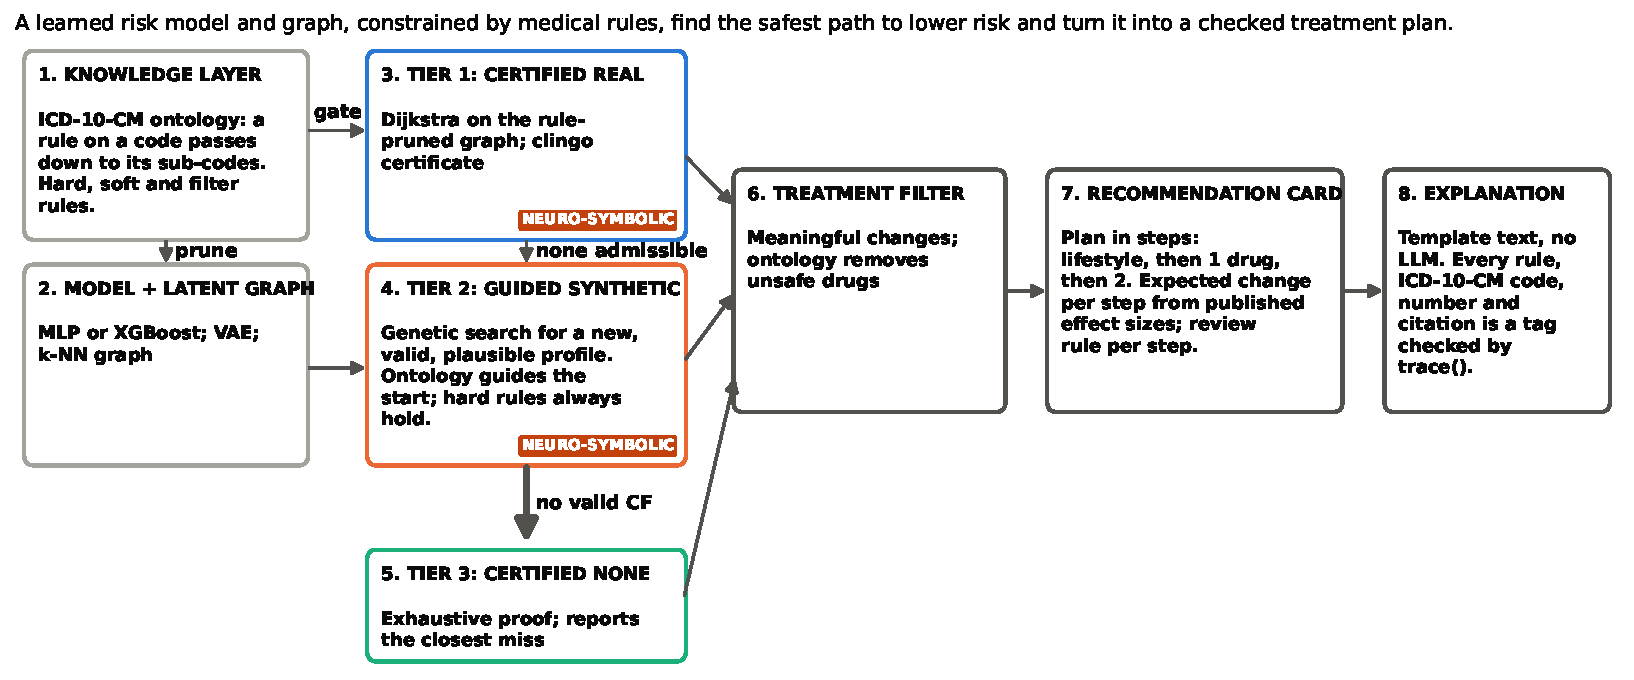
\includegraphics[width=0.62\textwidth]{figures/fig01_architecture_notitle.pdf}
  \caption{\method{} architecture. A dataset adapter supplies features, ICD-10-CM concepts and current medications. Tier~1 searches a rule-pruned graph over real training patients; tier~2 runs only when tier~1 is certified infeasible; tier~3 certifies that neither found admissible recourse. All tiers feed one recommendation and explanation stage.}
  \label{fig:arch}
\end{figure*}

\begin{figure}[t]
  \centering
  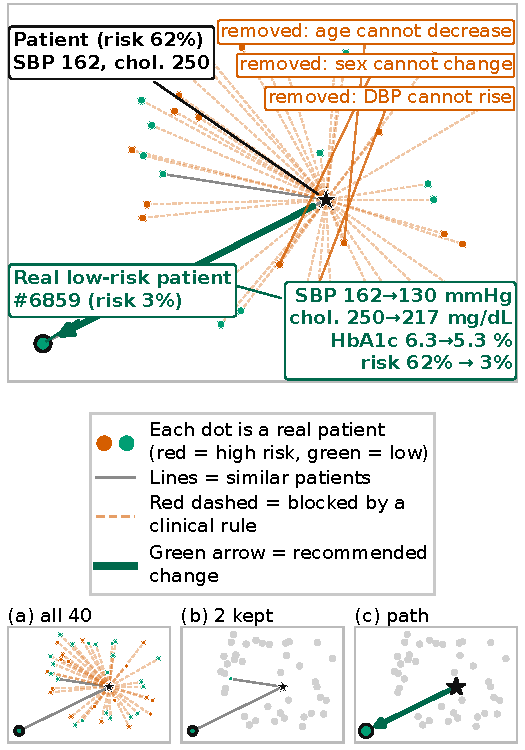
\includegraphics[width=\columnwidth]{figures/fig_calg_col.pdf}
  \caption{One patient in the rule-pruned latent graph (NHANES 1999--2023, seed 2, test patient 139, the patient of the example card). Each dot is a real patient: the 39 nearest training patients by Riemannian distance in the VAE latent space plus the certified target (patient 6859, farther away); red = PCE $\geq$ 7.5\%, green = lower risk. Layout: 2-D PCA of the latents (square-root distance compression; axes carry no meaning). Of the 40 similarity edges from the patient, the clinical rules remove 38 (dashed red, one rule labelled each) and keep 2; the thick green arrow is the recommended change (model risk 62\% to 3\%). Strip: (a) all neighbours, (b) after rule pruning, (c) chosen path.}
  \label{fig:calg}
\end{figure}

\subsection{Problem setting}
A patient $x$ has features of three classes: \emph{immutable} (sex), \emph{non-decreasing} (age) and \emph{mutable} with a direction (systolic and diastolic blood pressure, total cholesterol, BMI and HbA1c, all to be reduced). The adapter also supplies ICD-10-CM concepts $\mathcal{C}(x)$ and current intervention classes. An oracle $f$ (MLP or XGBoost~\cite{chen2016xgboost}, whichever has the higher validation AUC) gives risk $r_0=f(x)$; a patient is \emph{high-risk} if $r_0>0.55$. Because the PCE label is dominated by age, a single low-risk threshold is out of reach for most older patients, so the goal is age-stratified: $\tau(x)=\min(c_{a(x)},\,r_0)$, where $c_{a}$ is the bottom risk quartile within the patient's age quartile. A counterfactual $x'$ is \emph{valid} if $f(x')<\tau(x)$ and \emph{admissible} if it violates no hard rule.

\subsection{Knowledge layer}
One set of tables serves all datasets: 30 feature rules, 13 intervention classes in three escalation tiers (five lifestyle classes; single drugs: statin, ACE inhibitor/ARB, thiazide, calcium-channel blocker, non-selective beta-blocker, metformin, SGLT2 inhibitor, GLP-1 receptor agonist), and 18 contraindications attached to ICD-10-CM nodes, drafted from hypertension, cholesterol, prevention, diabetes, kidney and asthma guidelines~\cite{whelton2018htn,grundy2019chol,arnett2019prev,ada2024standards,kdigo2024ckd,gina2024}. \todo{all guideline rows are marked verify=1 in knowledge/citations.csv and must be checked}

For NHANES, survey answers and prescriptions become concepts: e.g.\ doctor-told diabetes $\to$ E11, asthma $\to$ J45.909, weak or failing kidneys $\to$ N18.9, BMI $\ge 30$ $\to$ E66.9, plus the ICD-10-CM reason codes recorded with prescriptions in 2013--2020. A rule attached at node $n$ applies if some concept in $\mathcal{C}(x)$ lies under $n$; for one feature the deepest attachment wins and ties take the envelope (Fig.~\ref{fig:onto}). Rules fall into three tiers:
\begin{itemize}
  \item \emph{Hard}: immutables equal; age never decreases and rises by at most 3.05 years along a tier-1 path; directional features never worsen beyond a per-feature measurement tolerance.
  \item \emph{Soft}: patient-specific target ranges (e.g.\ SBP below 130 under E08--E13, N18, I20--I25, I50 or Z86.73) and a maximum plausible change.
  \item \emph{Filter}: inherited contraindications (e.g.\ non-selective beta-blocker under J45, thiazide under M10, metformin under N18.4--N18.6) and indications (e.g.\ antihypertensives only above the patient-specific BP target).
\end{itemize}
All arithmetic uses integers scaled by 1000, so the clingo program and the vectorised NumPy mirror agree exactly; parity is 100\% on all datasets with and without inheritance.

\begin{figure}[t]
  \centering
  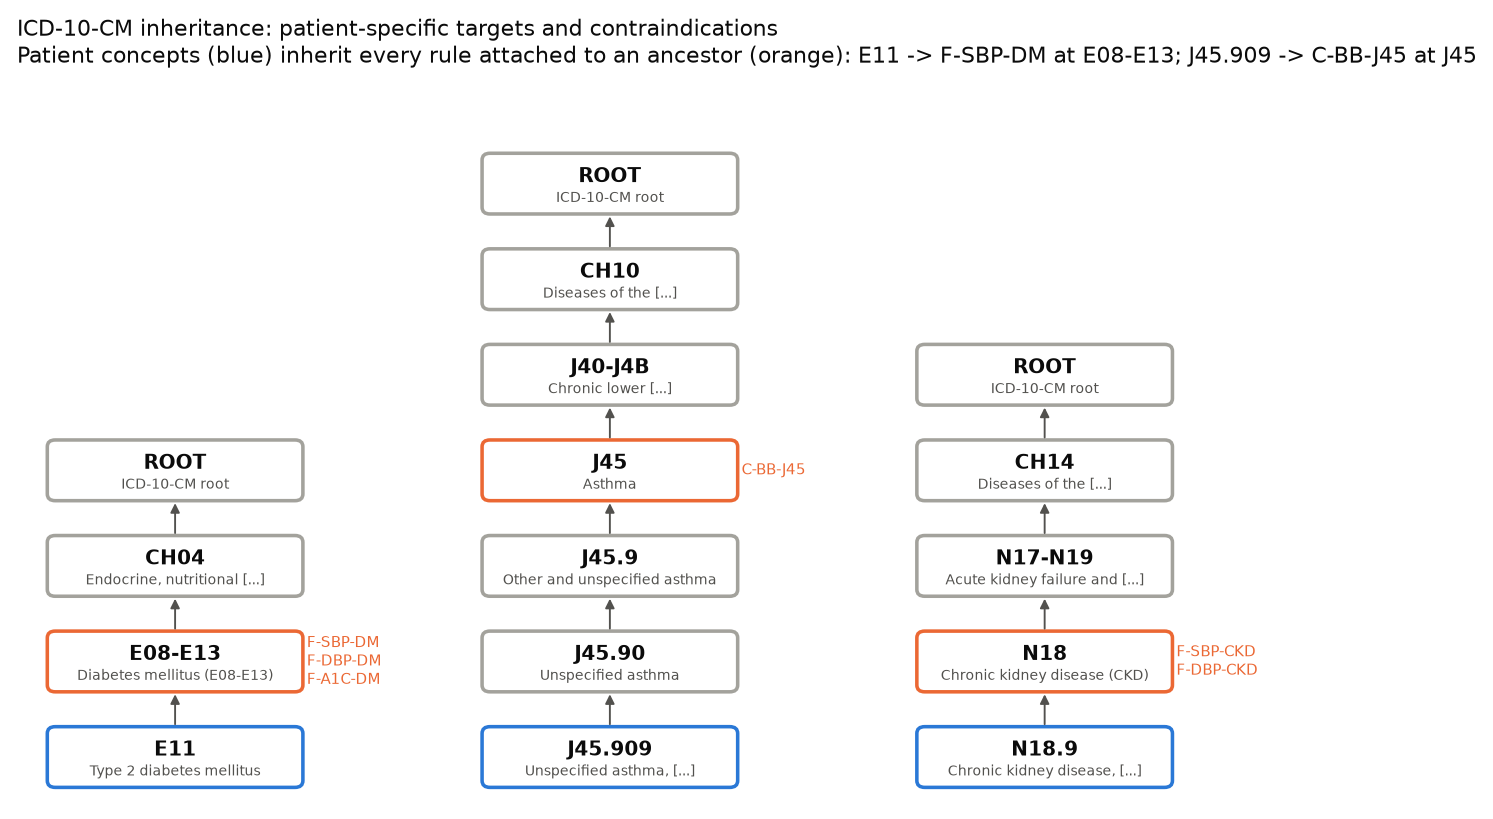
\includegraphics[width=0.7\columnwidth]{figures/fig03_ontology_inheritance.png}
  \caption{Inheritance. A patient concept (blue) inherits every rule attached at an ancestor (orange): E11 activates the diabetes BP and HbA1c targets at E08--E13; J45.909 activates the beta-blocker contraindication at J45; N18.9 activates the CKD BP targets at N18. \todo{remove in-image title}}
  \label{fig:onto}
\end{figure}

\subsection{Tier 1: certified real-patient recourse}
A type-aware VAE~\cite{kingma2014vae} (4-dimensional latent space, separate decoder heads per feature type) embeds all training patients. A $k$-nearest-neighbour graph ($k=120$ for pooled NHANES) is built in latent space; edges that violate the hard tier are pruned, and edge weights are Riemannian lengths under the decoder's pullback metric~\cite{arvanitidis2018oddity}. The query patient is attached to every training node through the same gate used for interior edges (\emph{gate symmetry}). Under \emph{source-relative admissibility} (SRA), every node on a path must be admissible from the source $x$ itself, not only from its predecessor, which prevents small admissible hops from adding up to an inadmissible change. Targets are training patients with $f<\tau(x)$; Dijkstra returns the shortest admissible path (Fig.~\ref{fig:calg}: for one patient the rules remove 38 of 40 neighbour edges). Every node is then re-checked on its \emph{recorded} values, not decoded ones, and clingo emits a certificate.

\begin{proposition}
With full query attachment and SRA, tier~1 succeeds if and only if some target is admissible directly from $x$. A tier-1 failure is therefore an exhaustive certificate that no real training patient is an admissible target.
\end{proposition}
\begin{IEEEproof}[Sketch]
If a target $t$ is admissible from $x$, the edge $x\to t$ exists by full attachment. Conversely, every node on an SRA path, including the endpoint, is admissible from $x$.
\end{IEEEproof}
The proposition was checked patient by patient (0 violations). The graph and metric therefore decide \emph{which} real patient is returned, not \emph{whether} one exists.

\subsection{Tier 2: ontology-guided synthetic counterfactuals}
For patients that tier~1 certifies infeasible, an elitist genetic search minimises a validity hinge to $\tau(x)$ plus MAD-scaled $L_1$ proximity, $L_0$ sparsity, the soft-rule penalty, a kNN plausibility term and a penalty on changes reachable only through contraindicated interventions, and returns three diverse counterfactuals. The hard tier holds by construction: sex and age are frozen, directional features move one way only, discrete features snap to their grid, and values stay within physiological bounds. \emph{Symbolic guidance} gives higher mutation probability to features that an allowed, indicated intervention can move, with steps directed toward the patient-specific target.

\subsection{Tier 3: certified none}
If tier~1 is certified infeasible and tier~2 finds no valid counterfactual, the patient receives no recommendation. The explanation states the best risk reachable if every mutable feature took its best recorded value and names the rules that block the closest real low-risk patient. A validity-only search with twice the budget separates \emph{model-ceiling} cases from guided-search misses (search-based, not a proof).

\subsection{Recommendations and explanations}
Changes above a minimum meaningful size map to intervention classes through \texttt{acts\_on} edges with matching direction. Contraindicated, non-indicated and already-taken classes are removed and listed. The remaining classes are ordered by escalation: lifestyle classes first with their typical guideline effect sizes, then the best single drug (first-line first), then a second drug; a drug counts as \emph{over-treatment} if lifestyle alone would cover every feature it addresses. A four-part template states why the risk is high (SHAP~\cite{lundberg2017shap}), what to change and which tier the target comes from, which interventions and why, and which rules applied. Every rule, node, intervention, citation, value and risk tag is machine-traced to the run's records.

% =====================================================================
\section{Experimental Setup}
% =====================================================================
\textbf{Data.} The primary cohort pools all eleven continuous NHANES cycles from 1999--2000 to August 2021--2023~\cite{nhanes}. From 119,555 participants, we keep adults aged 40--79 (the PCE range) with the examination, laboratory and questionnaire components and complete model features and HDL: 32,786. The label is PCE 10-year ASCVD risk $\ge$7.5\%~\cite{goff2014pce} (prevalence 49.9\%). Auscultatory (1999--2016) and oscillometric (2017--2023) blood pressure are averaged over available readings; analyses are unweighted. The 2019 linked mortality files cover 24,518 participants (1999--2018; 4,544 deaths, 1,329 cardiovascular; median follow-up 118 months). We also report NHANES 2017--2020 alone (4,539), UCI Heart~\cite{detrano1989} (297; angiographic disease) and Kaggle CVD-8k (an 8,000-patient stratified subsample of the Kaggle Cardiovascular Disease dataset~\cite{ulianova2019cardio}; recorded disease). UCI and CVD-8k have no concepts, so they use generic rules and ontology ablations are not applicable. % DATA_PROVENANCE_pooled.md, cohort_flow.csv

\textbf{Protocol.} Stratified 80/20 split, repeated over seeds 0--4. On pooled NHANES, models, VAE, graph and targets use all patients, and per-patient evaluation covers every high-risk test patient of each seed (15,002 in total; 2,931--3,073 per seed). All methods share the oracle, the per-patient goal $\tau(x)$ and the evaluator.

\textbf{Baselines.} FACE~\cite{poyiadzi2020face} (same target set and $k$), DiCE~\cite{mothilal2020dice}, Growing Spheres~\cite{laugel2018growing}, a PACE-style ASP-constrained search~\cite{pace2026}, C-CHVAE~\cite{pawelczyk2020cchvae}, and reachable-set verification~\cite{kothari2024reach} on a logistic-regression model (Wachter-style optimisation is not part of this comparison). C-CHVAE and the reachable-set verifier are faithful reimplementations because the reference libraries conflicted with our environment; deviations are documented in the code.

\textbf{Metrics.} Tier split and coverage (tier 1 + tier 2); \emph{valid and admissible} rate; real-value violations of tier-1 paths; contraindicated cards; escalation appropriateness and over-treatment; actionability; MAD-$L_1$ proximity, $L_0$ sparsity, LOF plausibility~\cite{breunig2000lof}; soft-rule violations; and validity after retraining the oracle with a new seed. We report mean $\pm$ SD over seeds and paired Wilcoxon tests with Holm correction~\cite{holm1979}.

% =====================================================================
\section{Results}\label{sec:results}
% =====================================================================
\subsection{Who receives recourse}
\begin{table}[t]
\centering
\caption{Tier split (\% of high-risk test patients, mean $\pm$ SD over 5 seeds). $n$: high-risk patients evaluated over all seeds.}
\label{tab:tiers}
\footnotesize
\setlength{\tabcolsep}{1.6pt}
\begin{tabular}{@{}lrcccc@{}}
\toprule
Dataset & $n$ & Tier 1 & Tier 2 & Tier 3 & Tier 1+2 \\
\midrule
NHANES 1999--2023 & 15,002 & \textbf{63.1}$\pm$2.8 & 33.2$\pm$10.1 & 3.6$\pm$7.9 & \textbf{96.4}$\pm$7.9 \\
NHANES 2017--2020 & 2,151 & 40.0$\pm$5.2 & 43.7$\pm$19.1 & 16.3$\pm$14.7 & 83.7$\pm$14.7 \\
UCI Heart & 115 & 26.0$\pm$9.4 & 69.8$\pm$8.4 & 4.2$\pm$6.0 & 95.8$\pm$6.0 \\
Kaggle CVD-8k & 3,296 & 98.8$\pm$0.7 & 1.2$\pm$0.6 & 0.1$\pm$0.1 & 99.9$\pm$0.1 \\
\bottomrule
\end{tabular}
\end{table}
% headline_tiered.csv, tier1_guarantees.csv


Table~\ref{tab:tiers} gives the tier split. On pooled NHANES, 63.1\% of high-risk patients receive a certified path to a real patient, 33.2\% a guided synthetic counterfactual and 3.6\% a certificate of infeasibility; 95.1\% receive a card with at least one allowed intervention. Both required guarantees held everywhere they were claimed: across 13,612 tier-1 paths on the four datasets, no node or endpoint violated a hard rule on recorded values and every clingo certificate passed, and no card in the main method contained a contraindicated class. Pooling matters: on the 2017--2020 cycle alone, tier~1 covers 40.0\%, and on pooled data tier-1 coverage rises with cohort size from 36.8\% (2k patients) through 41.7, 50.9 and 59.8\% to 63.1\% (all 32,786). Tier-1 paths are short (1.05 hops on average), consistent with the proposition. The mean risk drop to the target is 0.32. % pooled_learning_curve.csv

\emph{Seed variability.} The large SDs in Table~\ref{tab:tiers} (tier~2 $\pm$10.1, tier~3 $\pm$7.9 points) come from one seed. Per seed (tier 1/2/3, \%): 0 (MLP) 63.3/36.7/0.0; 1 (MLP) 64.8/35.0/0.2; 2 (XGBoost) 66.7/15.5/17.8; 3 (MLP) 60.5/39.5/0.0; 4 (MLP) 60.3/39.5/0.1. Only seed~2 selected XGBoost as oracle; its tier-3 patients are almost all model-ceiling cases (98.2\% of pooled tier~3; the validity-only search cannot push the risk below the goal), and its top age-bracket cut-off differs (0.981 vs.\ 0.996--0.998). With five seeds the oracle family and the seed are confounded, so we report rather than attribute the split.

\subsection{Comparison with baselines}
\begin{table*}[t]
\centering
\caption{Methods on pooled NHANES (15,002 high-risk patients, same oracle and per-patient goal). \emph{Valid}: reaches $\tau(x)$; \emph{admissible}: no hard-rule violation (immutables, age, directional non-worsening). \method{} exceeds every baseline on valid-and-admissible coverage (paired Wilcoxon, Holm $p<10^{-4}$).}
\label{tab:methods}
\footnotesize
\setlength{\tabcolsep}{4pt}
\begin{tabular}{@{}lcccccccc@{}}
\toprule
Method & Valid \% & Valid \& adm.\ \% $\uparrow$ & Hard viol.\ in valid \% $\downarrow$ & MAD-$L_1$ $\downarrow$ & $L_0$ $\downarrow$ & LOF $\downarrow$ & Action.\ $\uparrow$ & Soft viol.\ $\downarrow$ \\
\midrule
\textbf{\method{} (tiered)} & 96.4 & \textbf{96.4} & 0.0 & 9.18 & 4.26 & 1.31 & 0.94 & 2.62 \\
\quad tier 1 only (real) & 63.1 & 63.1 & 0.0 & 10.22 & 5.28 & 1.16 & 0.92 & 2.60 \\
\quad tier 2 only (guided GA) & 96.3 & 96.3 & 0.0 & 5.72 & 2.05 & 1.35 & 0.98 & 2.47 \\
\midrule
PACE-style~\cite{pace2026} & 66.4 & 66.4 & 0.0 & 4.22 & 5.87 & 1.32 & 0.96 & 2.12 \\
Reachable set (LR)~\cite{kothari2024reach} & 28.1 & 28.1 & 0.0 & 4.28 & 1.96 & 1.37 & 0.87 & 1.90 \\
DiCE~\cite{mothilal2020dice} & 81.4 & 12.0 & 85.1 & 11.76 & 5.98 & 2.34 & 0.73 & 4.00 \\
C-CHVAE~\cite{pawelczyk2020cchvae} & 49.1 & 9.9 & 79.7 & 6.86 & 5.96 & 1.01 & 0.71 & 2.43 \\
Growing Spheres~\cite{laugel2018growing} & 99.4 & 1.6 & 98.4 & 2.48 & 7.00 & 1.23 & 0.68 & 2.33 \\
FACE~\cite{poyiadzi2020face} & 100.0 & 0.4 & 99.6 & 4.39 & 6.04 & 1.06 & 0.60 & 2.22 \\
\bottomrule
\end{tabular}
\end{table*}
% methods_comparison.csv, methods_wilcoxon_holm.csv

Table~\ref{tab:methods} compares methods on pooled NHANES. Every baseline is valid for some patients, but FACE, Growing Spheres, DiCE and C-CHVAE reach the goal mostly by changing sex, lowering age or worsening a directional feature: 79.7--99.6\% of their valid counterfactuals are inadmissible. Among methods that respect the hard rules, the PACE-style search is strongest at 66.4\%; \method{} reaches 96.4\% (Holm $p<10^{-4}$ against each baseline). The ordering is the same on NHANES 2017--2020 (83.7\% vs.\ 62.1\% for PACE-style), UCI (95.8\% vs.\ 62.9\%) and CVD-8k (99.9\% vs.\ 69.8\% for PACE-style).

The table also shows the price of tier~1. Real targets are farther from the patient (MAD-$L_1$ 10.22 vs.\ 5.72 for tier~2) because a recorded person differs from the patient in more features, but they are more plausible (LOF 1.16 vs.\ 1.35) and far more robust: after retraining the oracle with a new seed, tier-1 targets remain valid for 84.9\% of patients against 63.5\% for tier-2 targets (89.8 vs.\ 48.0\% on NHANES 2017--2020). Tier~2 alone covers nearly as many patients as the tiered method, so the case for tier~1 is plausibility, robustness and the certificate, not coverage. The Riemannian natural-gradient variant of tier~2 reached only 24.6\%. % robustness_retraining.csv, tier2_variants.csv

\emph{Why \method{}'s MAD-$L_1$ (9.18) exceeds PACE-style's (4.22).} (i)~Each entry is a mean over a method's own valid counterfactuals, i.e.\ over different patients (PACE-style is valid for 66.4\% of patients, \method{} for 96.4\%). (ii)~Most \method{} counterfactuals are tier-1 targets, recorded people who differ in more features than a minimal synthetic edit (10.22 for tier~1 vs.\ 5.72 for tier~2). (iii)~On the 9,962 patients that both methods solve, \method{} still moves farther (paired mean difference $+2.73$, Holm $p<10^{-4}$) with fewer changed features ($L_0$ 4.26 vs.\ 5.87): the price of landing on a real, certified patient.

\subsection{Ablations}
% ablations.csv
\begin{figure*}[t]
  \centering
  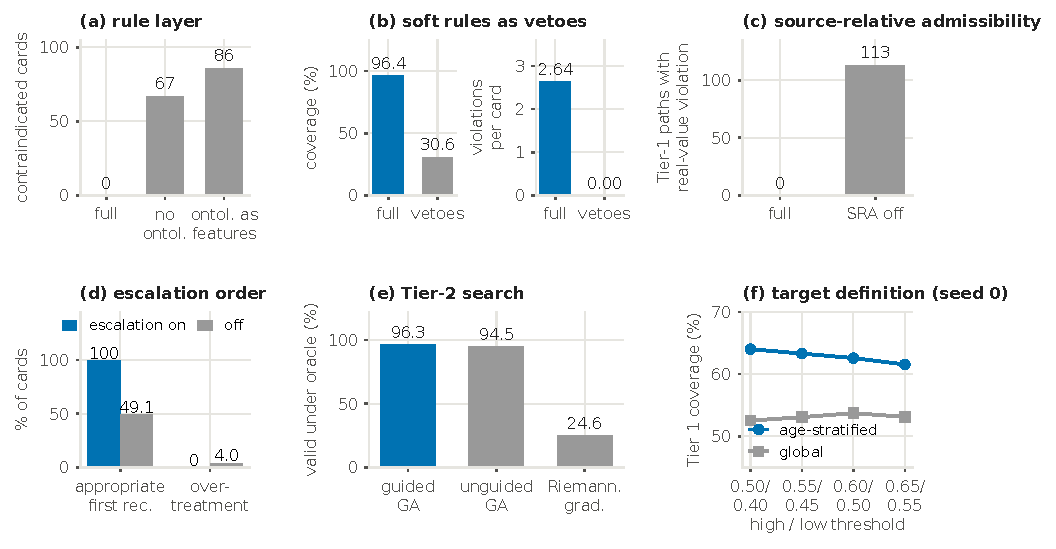
\includegraphics[width=0.72\textwidth]{figures/fig_ablation_grid.pdf}
  \caption{Ablations on pooled NHANES (15,002 high-risk patients, 5 seeds). (a)~Contraindicated cards. (b)~Soft rules as vetoes: coverage and violations per card. (c)~Tier-1 paths with a real-value violation without SRA. (d)~Escalation order. (e)~Tier-2 search validity. (f)~Age-stratified vs.\ global target, tier-1 coverage (seed 0).}
  \label{fig:abl}
\end{figure*}

Fig.~\ref{fig:abl} isolates the components. Without the ontology, or without inheritance, contraindicated recommendations reach the cards (67 and 69, i.e.\ 0.44\% and 0.45\%; 17 on NHANES 2017--2020) (mostly beta-blockers for asthma and thiazides for gout, whose rules reach the patient only through inheritance); coverage is unchanged.  Ranking by risk drop instead of escalation leaves only 49.1\% of cards guideline-ordered, and 4.0\% over-treat. Without SRA, 0.76\% of tier-1 paths (113 paths) (5.97\% on CVD-8k) carry a real-value violation, for a 0.6-point gain in tier-1 coverage. Soft rules as vetoes collapse coverage to 30.6\%. Symbolic guidance has a small but consistent effect: tier-2 validity 96.3 vs.\ 94.5\% on pooled data. Finally, using ICD-10-CM blocks as \emph{model features} (all 16,074 high-risk test patients) raises AUC (0.988 vs.\ 0.964) but cuts tier-1 coverage from 63.1\% to 14.6\%, because every indicator becomes an immutable feature, and contraindicated recommendations reappear (86, 0.53\% of cards). The ontology serves recourse better as rules than as features. A Euclidean metric changes paths but not coverage.

After oracle retraining, 84.9\% of tier-1 but 63.5\% of tier-2 recommendations remain valid. Age cannot decrease and sex cannot change block 96.8\% and 61.8\% of low-risk candidate targets, and are the closest miss for 2,741 and 2,089 of the 5,531 tier-1 failures.

\subsection{Predictor and external validity}
Test AUC is 0.964 for both models on pooled NHANES (0.959/0.960 on 2017--2020, 0.830/0.811 on UCI, 0.803/0.801 on CVD-8k, MLP/XGBoost); the MLP was chosen as oracle in four of five pooled seeds. The oracle's risk correlates with the PCE percentage (Spearman 0.92), and 92.6\% of gate-high patients have PCE $\ge$7.5\%. Against real outcomes, the PCE label discriminates linked cardiovascular death with AUC 0.782 and the oracle's risk reaches 0.774 on the seed-0 test set. Training on 1999--2016 and testing on 2017--2020 and 2021--2023 gives AUC 0.963 and 0.970 with tier-1 coverage of 64.4\% and 64.9\%; restricting to auscultatory BP cycles changes nothing (AUC 0.963). % model_metrics_summary.csv, pooled_mortality_validation.csv, pooled_cycle_held_out.csv

\textbf{The label and the oracle.} The PCE label is a formula of the inputs (age, sex, blood pressure, cholesterol and a few covariates), so a logistic regression on the seven model inputs already reaches test AUC 0.960 (MLP and XGBoost 0.964): the oracle reproduces a guideline equation rather than predicting outcomes. It stands in for any black-box risk model. The tiers, rules, certificates and recommendations use only its risk output and the recorded training patients, so the method itself does not depend on the label; only its evaluation does. The label is clinically meaningful: its AUC for linked cardiovascular death is 0.782.

\subsection{Certification and the reachable-set verifier}
All 5,531 pooled tier-1 failures are certified infeasible over every real training patient; 5.4\% are blocked only by the 3.05-year age horizon, and a hop-wise (non-SRA) two-hop chain would exist for 3.1\%. Of the 546 tier-3 patients, 98.2\% are model-ceiling cases. The reachable-set verifier on logistic regression flags 15.7\% of high-risk patients as precluded, yet 7.5\% of all high-risk patients are flagged precluded by it although \method{} finds certified real recourse for them (6.6\% guided recourse); it calls 2.0\% feasible where we end in tier~3, and its own counterfactuals are valid under the oracle only 28.1\% of the time: a linear verifier is not a safe proxy for a non-linear model. % certification.csv, reachable_set_head_to_head.csv

\subsection{Who is left without recourse}
Infeasibility is unevenly shared (patients pooled over seeds). Tier~1 reaches 89.5\% of high-risk women but 48.2\% of men ($\chi^2$ $p<10^{-100}$), in every seed (women 87.4--91.0\%, men 43.6--54.4\%). Tier-3 cases occur only in men (5.7\% pooled, none among women; 24.3\% vs.\ 0\% on 2017--2020), but the pooled figure comes almost entirely from seed~2 (27.2\% of men vs.\ 0.0--0.3\% elsewhere), so it should be read with the oracle sensitivity above. Tier~1 falls with age, from 83.5\% at 40--49 to 59.8\% at 70--79; tier~3 is 5.4--7.5\% at 40--69 and 0.2\% at 70--79. Race/ethnicity (tier~3 3.2--4.8\%) and cycle (3.0--4.4\%) differences are small. Blocking rules point to the mechanism: among tier-1 failures, age decrease blocks 97\% of candidate targets and sex 62\%. Young men are high-risk under the age-dominated PCE label while their age-bracket cut-off is very low, so few admissible targets exist. This is a property of the label and target definition, not of the search, and it should be shown to users rather than hidden. % fairness_tier_split.csv, blocking_rules.csv

% =====================================================================
\section{Limitations}
% =====================================================================
\textbf{(1) The goal is relative.} The age-stratified goal $\tau(x)=\min(c_{a},r_0)$ is weak in the oldest bracket, where $c_a\approx0.97$. Only 44.2\% of pooled targets fall below the global level of 0.45; with a global 0.45 goal tier-1 coverage is 52.5--53.7\% across thresholds (seed 0) instead of 61.6--64.0\%. \todo{total (tier 1+2) coverage under the global goal is not in the existing tables (they hold tier-1 coverage only); needs a tier-2 run with the global goal}
\textbf{(2) The oracle approximates a guideline equation;} linked mortality supports the label, but recourse targets the model, not the patient's outcome.
\textbf{(3) Soft floors.} Tier~1 enforces only hard rules, so real targets can overshoot soft guideline floors (2.6 soft violations per target on average; 11.5\% of tier-1 targets set SBP below the 90\,mmHg floor).
\textbf{(4) Observational.} Tier~1 compares a patient with a \emph{different} person; recommendations are not causal effects~\cite{prosperi2020causal}.
\textbf{(5) Knowledge provenance.} Every guideline row was drafted from memory and needs clinical review; diabetes type is unknown in NHANES and mapped to E11; 2021--2023 has no drug names; analyses are unweighted.
\textbf{(6) Scope.} Explanation texts (with SHAP) are stored for the first 60 patients per seed, two baselines (C-CHVAE, reachable set) are reimplementations, and the oracle family changes the tier-2/3 split.

% =====================================================================
\section{Conclusion}
% =====================================================================
\method{} gives nearly every high-risk patient in a large population cohort either admissible, guideline-ordered and contraindication-free recourse or an honest certificate that none exists, with certified real targets for most. Ontology inheritance keeps unsafe drugs off the cards, source-relative admissibility keeps real paths free of drift, and real-patient targets are markedly more robust to model retraining than synthetic ones. Next: a MIMIC-IV adapter~\cite{johnson2023mimiciv} and clinician review. \todo{code availability link}

\section*{Acknowledgment}
\todo{acknowledgments; NHANES public-use data statement}

\bibliographystyle{IEEEtran}
\bibliography{refs}

\end{document}
